\chapter{Métodos e materiais}
\label{cap:metodologia}

O Capítulo~\ref{cap:contexto} estabeleceu que as três perguntas do investidor particular têm
resposta na literatura mas não em nenhuma ferramenta gratuita. Este capítulo descreve as opções
tomadas para lhes responder. Apresenta-se primeiro a metodologia de investigação e os conjuntos de
dados. Descrevem-se em seguida os quatro métodos selecionados, um para cada decisão que o sistema
tem de tomar. Indicam-se as ferramentas empregues. E enunciam-se, por fim, os desafios tecnológicos
e sociais do domínio.

\section{Metodologia de investigação}
\label{sec:met_metodologia}

Esta dissertação enquadra-se na investigação por desenho \autocite{hevner2004design}, na qual o
objeto de estudo é um artefacto construído para resolver uma classe de problema e o conhecimento
produzido reside tanto no artefacto como no processo da sua avaliação. Trata-se do enquadramento
adequado quando a contribuição é um sistema, e distingue-se de um estudo puramente empírico pelo
facto de o objeto avaliado não existir antes da sua construção.

A literatura de investigação por desenho estabelece que a avaliação do artefacto deve ser rigorosa
e constituir uma atividade central do processo, e não um passo final de confirmação
\autocite{hevner2004design, peffers2007dsrm}. Este requisito é cumprido através de três
compromissos assumidos antes da execução das experiências.

O primeiro consiste em comparar cada componente com uma alternativa mais simples, selecionada e
declarada antes de a medição ser realizada, de modo que o resultado possa ser negativo. O segundo
consiste em fixar o critério de sucesso de cada comparação juntamente com a métrica, e não após a
observação dos valores obtidos. O terceiro consiste em avaliar o artefacto duas vezes: sobre dados
históricos retidos e, posteriormente, em funcionamento, sobre as decisões que o sistema toma
autonomamente em produção. A terceira avaliação é a menos comum das três e é a que produz o
resultado descrito na Secção~\ref{sec:av_producao}.

A exigência não é cumprida na totalidade, e a lacuna é declarada. Utilidade, no sentido em que a
literatura de investigação por desenho emprega o termo, é utilidade para quem usa o artefacto, e
essa propriedade determina-se com utilizadores. O que nesta dissertação foi medido é a fidelidade
das explicações produzidas, propriedade que pertence ao sistema; a utilidade, que depende da
relação entre o sistema e quem o lê, permanece por medir.

O sistema toma quatro decisões distintas, representadas na Figura~\ref{fig:met_decisoes}. As três
primeiras correspondem às questões enunciadas no Capítulo~\ref{cap:introducao}; a quarta não é uma
questão do investidor, mas do próprio sistema, e existe porque responder às três primeiras não
implica interromper o utilizador.

\begin{figure}[ht]
\centering
\begin{tikzpicture}[
  font=\small, >={Stealth[length=2.4mm]},
  cx/.style={draw, rounded corners, align=center, text width=2.85cm, minimum height=2.0cm,
             inner sep=4pt, fill=black!4},
  num/.style={font=\bfseries\small, text=black!45},
]
  \node[cx] (a) {\textbf{1. É invulgar?}\\[3pt]
    \footnotesize comparar hoje com o\\ \footnotesize normal \emph{desta} empresa};
  \node[cx, right=0.6cm of a] (b) {\textbf{2. Empresa ou}\\\textbf{mercado?}\\[3pt]
    \footnotesize repartir o movimento\\ \footnotesize pelas suas fontes};
  \node[cx, right=0.6cm of b] (c) {\textbf{3. Já aconteceu?}\\[3pt]
    \footnotesize procurar casos passados\\ \footnotesize e medir o que se seguiu};
  \node[cx, right=0.6cm of c] (d) {\textbf{4. Merece avisar?}\\[3pt]
    \footnotesize decidir se isto justifica\\ \footnotesize interromper alguém};
  \node[num, above=1mm of a] {estatística};
  \node[num, above=1mm of b] {regressão};
  \node[num, above=1mm of c] {significado};
  \node[num, above=1mm of d] {aprendizagem};
  \draw[->, thick, black!50] (a) -- (b);
  \draw[->, thick, black!50] (b) -- (c);
  \draw[->, thick, black!50] (c) -- (d);
\end{tikzpicture}
\caption[As quatro decisões do sistema]{As quatro decisões do sistema e a família de técnicas
associada a cada uma. As três primeiras correspondem às perguntas enunciadas no
Capítulo~\ref{cap:introducao}. A cada coluna corresponde uma secção deste capítulo, entre a
Secção~\ref{sec:met_detecao} e a Secção~\ref{sec:met_triagem}.}
\label{fig:met_decisoes}
\end{figure}


\section{Conjuntos de dados}
\label{sec:met_dados}

Esta secção descreve os conjuntos de dados utilizados no treino e na avaliação do sistema, bem
como os registos produzidos pelo sistema em funcionamento.

A camada histórica assenta no \gls{FNSPID} \autocite{dong2024fnspid}, um corpus público de notícias
financeiras que associa a cada título uma data e uma empresa. O corpus não contém preços, reação de mercado nem qualquer indicação de
relevância: essa informação é construída neste trabalho, alinhando cada título com as séries de
preços correspondentes. Do alinhamento resulta o conjunto de treino do modelo de triagem, com
79\,753 exemplos.

A avaliação do detetor de anomalias utiliza um conjunto distinto, composto por três anos de
cotações diárias. A escolha de um conjunto próprio é deliberada: a avaliação exige variedade de
volatilidade entre empresas, ao passo que a lista monitorizada em produção é uma decisão de
produto. Avaliar o detetor exatamente sobre o conjunto que ele foi construído para servir
produziria uma medição sem valor informativo.

Todos os preços utilizados são fechos ajustados para desdobramentos e distribuição de dividendos.
O ajuste não é um pormenor no período considerado, que contém um desdobramento de quatro para um
da Apple e dois da Tesla: sobre séries não ajustadas, o detetor assinalaria quedas de trinta a
oitenta por cento em dias sem qualquer acontecimento.

A Tabela~\ref{tab:met_conjuntos} reúne os conjuntos utilizados, e a
Tabela~\ref{tab:met_universos} os conjuntos de empresas, cujas contagens diferem por razões
descritas na coluna respetiva.

\begin{table}[!htbp]
\caption[Conjuntos de dados utilizados]{Conjuntos de dados utilizados no trabalho, com o intervalo
temporal e a dimensão lidos dos ficheiros. As três últimas linhas correspondem ao sistema em
funcionamento.}
\label{tab:met_conjuntos}
\centering
\small
\begin{tabular}{L{0.30\textwidth} L{0.26\textwidth} L{0.34\textwidth}}
\toprule
\tabhead{Conjunto} & \tabhead{Intervalo} & \tabhead{Dimensão} \\
\midrule
\multicolumn{3}{l}{\emph{Histórico}} \\
Conjunto de treino da triagem & 2018-01-02 a 2023-12-18 & $79\,753$ exemplos, 14 empresas \\
Preços para avaliação da deteção & 2023-06-01 a 2026-06-01 & 15 empresas, $\approx 750$ dias cada \\
\midrule
\multicolumn{3}{l}{\emph{Operação}} \\
Base de precedentes implantada & um ano de recolha própria & $38\,214$ casos com impacto medido \\
Alertas entregues & 2026-07-09 a 2026-08-13 & 367 mensagens \\
Registo de decisões de triagem & 2026-07-22 a 2026-08-15 & $4\,366$ decisões \\
\bottomrule
\end{tabular}
\end{table}

\begin{table}[!htbp]
\caption[Conjuntos de empresas]{Conjuntos de empresas utilizados. As contagens diferem porque cada
conjunto serve um propósito distinto. Os conjuntos não são encaixados: a lista monitorizada em
produção contém duas empresas ausentes de todos os conjuntos históricos.}
\label{tab:met_universos}
\centering
\small
\begin{tabular}{L{0.30\textwidth} C{0.10\textwidth} L{0.48\textwidth}}
\toprule
\tabhead{Conjunto} & \tabhead{Empresas} & \tabhead{Propósito} \\
\midrule
Mapa de setores alargado & 17 & Universo percorrido pela decomposição do movimento \\
Mapa canónico do histórico & 15 & Rótulo de relevância na avaliação da recuperação \\
Preços para a deteção & 15 & Variedade de volatilidade na avaliação do detetor \\
Conjunto de dados da triagem & 14 & Resultado do alinhamento entre notícias e preços \\
\quad coberto pelo bloco de treino & 13 & Empresas efetivamente presentes no treino \\
\quad coberto pelo bloco de teste & 9 & Empresas presentes na avaliação \\
Lista monitorizada em produção & 12 & Decisão de produto \\
\bottomrule
\end{tabular}
\end{table}

\section{Deteção de movimentos invulgares}
\label{sec:met_detecao}

A primeira decisão do sistema consiste em determinar se o movimento observado num dia é invulgar
para a empresa em causa. Uma regra de limiar fixo, do tipo assinalar variações superiores a três
por cento, é inadequada para este fim, porque a mesma percentagem corresponde a acontecimentos de
raridade muito distinta consoante a volatilidade da empresa.

O método adotado pertence à família estatística da taxonomia de deteção de anomalias
\autocite{chandola2009anomaly}, que define normalidade a partir da distribuição recente dos
próprios dados. O movimento do dia é comparado com o comportamento recente da mesma ação e
expresso em desvios-padrão:

\begin{equation}
z_t = \frac{r_t - \mu}{\sigma}
\label{eq:zscore}
\end{equation}

onde $r_t$ é o retorno logarítmico do dia, $r_t = \ln(P_t / P_{t-1})$, e $\mu$ e $\sigma$ são a
média e o desvio-padrão dos retornos dos vinte dias anteriores. A utilização de retornos
logarítmicos segue a convenção corrente em séries financeiras, por tornar os retornos aditivos ao
longo do tempo e simétricos entre subidas e descidas. Os valores apresentados diferem, por essa
razão, dos exibidos por uma aplicação de bolsa: um retorno logarítmico de $+19{,}82\%$ corresponde
a uma variação de preço de $+21{,}92\%$.

A janela desliza a cada dia, e o dia avaliado é excluído da janela que define a sua própria norma,
como representado na Figura~\ref{fig:met_janela}. Sem esta exclusão, o dia contribuiria para a
média e para o desvio-padrão contra os quais é comparado, atenuando a sua própria anomalia. A
mesma disciplina impede a utilização de qualquer informação posterior ao dia avaliado.

\begin{figure}[ht]
\centering
\begin{tikzpicture}[font=\small, >={Stealth[length=2.2mm]}]
  % barras dos dias
  \foreach \i in {0,...,19} {
    \fill[black!18] (\i*0.32,0) rectangle (\i*0.32+0.24,0.55);
  }
  \fill[orange!70] (20*0.32,0) rectangle (20*0.32+0.24,1.25);
  \draw[decorate, decoration={brace, amplitude=5pt}, black!55]
    (0,-0.15) -- (19*0.32+0.24,-0.15)
    node[midway, below=6pt, align=center, black!65]
    {\footnotesize os \textbf{20 dias anteriores}\\[-2pt]\footnotesize dão o $\mu$ e o $\sigma$};
  \draw[decorate, decoration={brace, amplitude=5pt}, orange!75!black]
    (20*0.32,-0.15) -- (20*0.32+0.24,-0.15)
    node[midway, below=6pt, align=center, text=orange!60!black]
    {\footnotesize o dia\\[-2pt]\footnotesize \textbf{a julgar}};
  \draw[->, thick, black!45] (20*0.32+0.6,0.6) -- (20*0.32+1.5,0.6)
    node[right, align=left, black!60] {\footnotesize amanhã a janela\\[-2pt]\footnotesize desliza um dia};
\end{tikzpicture}
\caption[A janela deslizante do \emph{z}-score]{A janela que estabelece o comportamento habitual da
ação. O dia avaliado \textbf{fica de fora} do cálculo da norma contra a qual é comparado, separação
que impede a utilização de informação indisponível no momento da decisão.}
\label{fig:met_janela}
\end{figure}

Quando o desvio-padrão da janela é nulo, a Equação~\ref{eq:zscore} não está definida. O sistema
distingue dois casos: a manutenção do valor constante não constitui anomalia, ao passo que um
afastamento dessa norma plana é assinalado sem lhe ser atribuído um valor de $z$, indicando-se que
a variância anterior era nula. Esta distinção evita que a proteção contra a divisão por zero
silencie precisamente o primeiro movimento após um período constante.

A aplicação do método ao maior movimento do período estudado, registado pela Tesla a 24 de outubro
de 2024, produz um retorno diário de $+19{,}82\%$ contra uma média de $-0{,}92\%$ e um
desvio-padrão de $2{,}72\%$ nos vinte dias anteriores, o que corresponde a $z = +7{,}61$. O valor
não decorre da dimensão absoluta do movimento, mas do facto de este exceder em sete vezes e meia a
oscilação habitual da ação naquelas semanas.


\section{Decomposição do movimento observado}
\label{sec:met_decomposicao}

A técnica anterior quantifica a dimensão do movimento, mas não identifica a sua origem. A segunda
decisão do sistema consiste em repartir o retorno observado nas suas componentes de mercado, de
setor e específica da empresa:

\begin{equation}
r = \underbrace{\beta_m r_m}_{\text{mercado}} + \underbrace{\beta_s \tilde{r}_s}_{\text{setor}} + \underbrace{\varepsilon}_{\text{empresa}}
\label{eq:decomposicao}
\end{equation}

As variáveis $r_m$ e $\tilde{r}_s$ designam, respetivamente, o retorno diário do índice de mercado
e o do setor, ao passo que $\beta_m$ e $\beta_s$ quantificam a sensibilidade histórica da ação a
cada uma dessas fontes. A componente específica da empresa é
definida como o resíduo, pelo que a soma das três parcelas reproduz sempre o movimento observado.
O mercado é representado pelo fundo cotado que segue o índice largo norte-americano, e o setor
pelo fundo setorial correspondente, escolhidos por serem os mais líquidos da sua classe e por
disporem de histórico longo em fontes gratuitas.

Três aspetos determinam a validade da repartição.

O primeiro é a ortogonalização do fator setorial. Um fundo setorial e o índice de mercado
apresentam movimentos fortemente correlacionados, e a sua introdução conjunta na regressão produz
coeficientes instáveis por colinearidade. O fator utilizado não é, por isso, o retorno do setor,
mas o resíduo de uma primeira regressão do setor sobre o mercado.

O segundo é a restrição temporal da estimação. A janela termina no dia anterior ao dia explicado,
pela mesma disciplina aplicada à deteção.

O terceiro é o tratamento do ruído. Uma sensibilidade estimada sobre vinte observações é imprecisa,
e estimativas extremas em janelas agitadas produzem repartições sem significado. A literatura de
finanças documenta que os betas estimados regridem para a média entre períodos sucessivos
\autocite{blume1971risk}, do que decorreu a prática de encolher a estimativa com um peso fixo. Essa
prática aplica a mesma correção a estimativas precisas e imprecisas. A alternativa adotada pondera
o encolhimento pela imprecisão da própria estimativa \autocite{vasicek1973beta}:

\begin{equation}
\beta = w \hat{\beta} + (1-w)\,\beta_{\text{ref}}, \qquad w = \frac{\sigma^2_{\text{ref}}}{\sigma^2_{\text{ref}} + \mathrm{SE}^2(\hat{\beta})}
\label{eq:vasicek}
\end{equation}

Quando o ajuste é preciso, o erro-padrão é reduzido, $w$ aproxima-se da unidade e a estimativa é
praticamente preservada; quando a janela é ruidosa, o erro-padrão cresce e a estimativa recai sobre
o valor de referência. O ajuste é gradual e não dicotómico. A formulação original estima
$\beta_{\text{ref}}$ e $\sigma^2_{\text{ref}}$ a partir da distribuição transversal dos betas;
neste trabalho são escolhas do autor, com $\beta_{\text{ref}} = 1{,}0$ para o mercado,
$\beta_{\text{ref}} = 0{,}0$ para o fator setorial já ortogonalizado, e um desvio-padrão comum de
$0{,}5$. A amostra de empresas não constitui um corte transversal representativo, pelo que a
estimação de um prior sobre ela produziria um valor com aparência empírica sem o ser.

Três salvaguardas completam a estimação. Abaixo de dez observações utilizáveis a regressão não é
tentada, assumindo-se sensibilidade unitária ao mercado e nula ao setor, situação que é declarada
ao utilizador. Uma estimativa cujo módulo exceda dez é tratada como falha numérica da janela e não
como sensibilidade económica, recaindo no mesmo recuo; a guarda destina-se a janelas degeneradas e
não substitui o encolhimento, que é o mecanismo que trata o ruído. Por fim, o termo constante é
recalculado sobre os coeficientes já encolhidos, uma vez que o valor devolvido pela regressão está
centrado nos coeficientes brutos e a sua reutilização descentraria o modelo efetivamente reportado.

A Figura~\ref{fig:met_decomposicao} apresenta a repartição de um movimento real, em que as
componentes de mercado e de setor atuam em sentido contrário ao movimento observado.

\begin{figure}[ht]
\centering
\begin{tikzpicture}[font=\small, >={Stealth[length=2.2mm]}, x=1cm, y=1cm]
  % escala: 1 cm = 1 ponto percentual. Os valores sao os do caso real da AMD.
  \def\yzero{0}
  \draw[black!30] (-0.4,\yzero) -- (10.6,\yzero);
  \node[left, font=\footnotesize, black!55] at (-0.45,\yzero) {$0\%$};

  % mercado: -0.3992
  \fill[black!45] (0.35,\yzero) rectangle (1.45,-0.40);
  \node[font=\footnotesize, align=center] at (0.9,-0.95) {mercado\\ $-0.40\%$};

  % setor: -0.0362 (quase invisivel, e isso e a informacao)
  \fill[black!45] (2.35,\yzero) rectangle (3.45,-0.04);
  \node[font=\footnotesize, align=center] at (2.9,-0.95) {setor\\ $-0.04\%$};

  % empresa: +6.7298
  \fill[black!70] (4.35,\yzero) rectangle (5.45,6.73);
  \node[font=\footnotesize, align=center, text=black] at (4.9,7.25) {\textbf{empresa}\\ $+6.73\%$};

  % soma observada
  \draw[black!25, dashed] (6.1,\yzero) -- (6.1,6.9);
  \fill[black!15, draw=black!55] (7.05,\yzero) rectangle (8.15,6.29);
  \node[font=\footnotesize, align=center] at (7.6,6.85) {movimento\\ observado\\ $+6.29\%$};

  \draw[->, black!55] (5.6,3.2) -- (6.9,3.2);
  \node[font=\footnotesize, black!55, align=center] at (6.25,2.6) {somam};

  \node[font=\footnotesize, black!60, align=left, text width=2.1cm]
    at (9.6,3.4) {as três parcelas somam ao movimento do dia, sempre};
\end{tikzpicture}
\caption[Um movimento repartido em três parcelas]{Repartição de um dia da AMD, o de 15 de agosto de
2026, em retornos logarítmicos. As componentes de mercado e de setor atuaram em sentido
descendente, pelo que a subida é integralmente atribuída à empresa. A igualdade entre a soma das
parcelas e o movimento observado verifica-se por construção e, por essa razão, nada estabelece
quanto à qualidade do ajuste, ponto retomado na Secção~\ref{sec:av_decomposicao}.}
\label{fig:met_decomposicao}
\end{figure}

Neste caso, registado pela AMD a 15 de agosto de 2026, o retorno logarítmico de $+6{,}2944\%$,
correspondente a uma variação simples do preço de $+6{,}50\%$, reparte-se em $-0{,}3992\%$ de mercado, $-0{,}0362\%$ de setor e $+6{,}7298\%$ específicos da
empresa, com $\beta_m = 2{,}0143$ e $\beta_s = 1{,}5888$ estimados sobre os vinte dias anteriores.
A informação transmitida excede a percentagem isolada: a ação subiu apesar de o contexto ter
atuado em sentido contrário, e o beta de mercado indica uma ação que historicamente amplifica os
movimentos do índice.

A soma exata das três parcelas não constitui validação do método. A igualdade verifica-se por
construção, uma vez que a componente específica é definida como resíduo, e uma repartição sem
significado somaria igualmente. A medida informativa sobre a qualidade do ajuste é o coeficiente
de determinação na janela de estimação, cujo valor é reportado no Capítulo~\ref{cap:avaliacao}.

\section{Recuperação de precedentes}
\label{sec:met_recuperacao}

A terceira decisão consiste em identificar notícias passadas comparáveis com a notícia em análise
e medir o comportamento subsequente do preço. A procura por correspondência de palavras é
inadequada por duas razões simétricas: notícias com o mesmo significado podem não partilhar
vocabulário, e notícias com vocabulário comum podem tratar de assuntos distintos.

A representação adotada é um modelo de embeddings de frase \autocite{reimers2019sbert}, que
converte cada título num vetor de 384 dimensões cuja posição no espaço reflete o significado da
frase. A contribuição relevante deste modelo não é a arquitetura, mas o objetivo de treino: os
vetores são aprendidos de modo que a distância entre dois deles corresponda a semelhança de
sentido. Um codificador da mesma família treinado para outra tarefa não herda esta propriedade,
observação que o Capítulo~\ref{cap:avaliacao} confirma experimentalmente.

A proximidade entre duas frases é medida pela semelhança do cosseno, ou seja pelo ângulo entre os
vetores e não pela distância entre as suas extremidades, o que torna a medida independente do
comprimento do texto. Os vetores são devolvidos com norma unitária, pelo que o cosseno se reduz ao
produto interno, propriedade que permite percorrer a base de casos completa sem aproximação. Sobre
dois pares reais da base de casos, dois títulos sobre a descida de empresas de tecnologia e
semicondutores obtêm $\cos = +0{,}956$, e um título sobre a Peloton comparado com outro sobre o
impacto da pandemia na indústria automóvel obtém $\cos = -0{,}086$. O limiar de semelhança
utilizado em produção é de $0{,}45$.

A ordenação dos candidatos não é, contudo, o cosseno isolado. Casos próximos no tema mas distantes
no tempo descrevem um regime de mercado que já não é o vigente, pelo que a ordenação aplica um
decaimento exponencial sobre a idade do caso, na forma $\cos \times 2^{-\text{idade}/h}$, com
meia-vida $h$ de cento e vinte dias. Um caso com um ano entra assim com peso aproximado de $0{,}12$
e prevalece apenas na ausência de material mais recente sobre o mesmo tema.

O decaimento ordena e
não é apresentado: o valor exibido junto de cada precedente é sempre o cosseno, uma vez que
apresentar uma pontuação composta sob o nome de semelhança produziria um número que o utilizador
não pode verificar. As duas decisões compõem-se em série, pelo que o limiar de $0{,}45$ incide sobre
um conjunto já selecionado pela ordenação, e não sobre os vizinhos de maior cosseno. A Figura~\ref{fig:met_embeddings} representa a propriedade que
esta medida explora: títulos com o mesmo significado ocupam posições próximas ainda que não
partilhem vocabulário, ao passo que títulos que partilham vocabulário e tratam de assuntos distintos
ficam afastados.

\begin{figure}[ht]
\centering
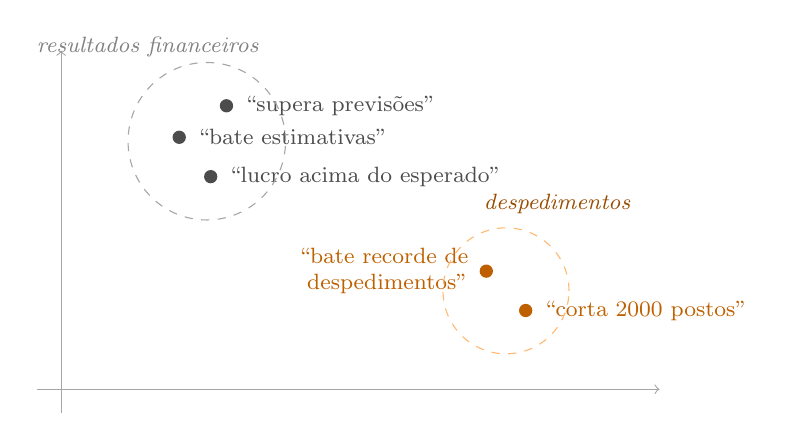
\begin{tikzpicture}[font=\small]
  \draw[->, black!35] (-0.3,0) -- (7.6,0);
  \draw[->, black!35] (0,-0.3) -- (0,4.3);
  % cluster resultados
  \fill[black!70] (1.5,3.2) circle (2.4pt) node[right=3pt, align=left, font=\footnotesize] {``bate estimativas''};
  \fill[black!70] (2.1,3.6) circle (2.4pt) node[right=3pt, align=left, font=\footnotesize] {``supera previsões''};
  \fill[black!70] (1.9,2.7) circle (2.4pt) node[right=3pt, align=left, font=\footnotesize] {``lucro acima do esperado''};
  \draw[black!35, dashed] (1.85,3.15) circle (1.0);
  \node[black!50, font=\footnotesize\itshape] at (1.1,4.35) {resultados financeiros};
  % cluster despedimentos
  \fill[orange!75!black] (5.9,1.0) circle (2.4pt) node[right=3pt, align=left, font=\footnotesize] {``corta 2000 postos''};
  \fill[orange!75!black] (5.4,1.5) circle (2.4pt) node[left=3pt, align=right, font=\footnotesize] {``bate recorde de\\ despedimentos''};
  \draw[orange!55, dashed] (5.65,1.25) circle (0.8);
  \node[orange!60!black, font=\footnotesize\itshape] at (6.3,2.35) {despedimentos};
\end{tikzpicture}
\caption[Frases como pontos num espaço]{Cada frase corresponde a um ponto do espaço. Frases de
significado próximo ocupam posições vizinhas ainda que não partilhem vocabulário, ao passo que
frases com vocabulário comum (``bate'') e assunto distinto ficam afastadas. A representação é
bidimensional para permitir a leitura; o modelo utiliza 384 dimensões.}
\label{fig:met_embeddings}
\end{figure}

A medição do desfecho adapta o estudo de evento \autocite{brown1985daily}: fixado o dia da notícia,
mede-se a variação do preço a um, três e cinco dias. Duas decisões de detalhe condicionam o
resultado. Notícias publicadas fora de dias de negociação são alinhadas com o primeiro dia de
negociação seguinte. A medição inicia-se no fecho do dia da notícia, e não na abertura, opção
conservadora que evita atribuir à notícia a parte do movimento anterior à sua publicação.

O valor apresentado ao utilizador é o retorno bruto e não o retorno anormal que a fonte
normaliza. A opção é deliberada e tem um custo declarado. O retorno bruto é verificável pelo utilizador na
sua própria aplicação, mas incorpora o movimento do mercado no período. Em períodos de queda
generalizada, os precedentes aparentam desfechos piores do que os atribuíveis à notícia. O desconto do mercado é aplicado onde é indispensável, na construção do
rótulo descrito na secção seguinte.


\section{Triagem de notícias}
\label{sec:met_triagem}

A quarta decisão determina que notícias justificam a interrupção do utilizador. Ao contrário das
anteriores, não dispõe de uma formulação analítica evidente, constituindo o ponto natural para
aprendizagem a partir dos dados.

O rótulo formaliza a pergunta como a ocorrência de um movimento anormalmente grande após a
notícia. Mede-se o retorno da ação nos três dias seguintes, subtrai-se o movimento do mercado no
mesmo período e classifica-se o exemplo como positivo quando o valor absoluto do resíduo excede
dois por cento. O uso do valor absoluto é deliberado: o modelo aprende sobre materialidade e nunca
sobre direção, o que preserva a restrição fundadora do trabalho.

A subtração do movimento do mercado assume uma sensibilidade unitária, o que constitui uma
incoerência com a técnica descrita na Secção~\ref{sec:met_decomposicao}, que recusa precisamente
essa suposição. Numa ação de beta elevado, o resíduo retém parte do movimento do mercado, e o
rótulo pode classificar como material um dia em que apenas o mercado se moveu. Todas as famílias de
modelos avaliadas no Capítulo~\ref{cap:avaliacao} são treinadas e avaliadas contra o mesmo rótulo,
pelo que a comparação entre elas é internamente consistente sob esta definição de alvo. Tal não
garante, porém, que a ordenação resista a uma definição alternativa, uma vez que o erro introduzido
pode estar correlacionado com a empresa e com a volatilidade.

O modelo recebe nove entradas: a volatilidade dos vinte dias anteriores, o momento dos cinco dias
anteriores, o retorno do próprio dia, o comprimento do título e cinco indicadores de setor. Uma
variante adicional incorpora o vetor de 384 dimensões do título. A Figura~\ref{fig:met_entradas}
agrupa as entradas pelo nível de informação que cada uma descreve, distinção que o
Capítulo~\ref{cap:avaliacao} demonstra ser determinante.

\begin{figure}[ht]
\centering
\begin{tikzpicture}[font=\footnotesize, >={Stealth[length=2mm]},
  cx/.style={draw, rounded corners=2pt, align=center, inner sep=3pt, minimum height=0.62cm,
             text width=2.35cm},
  emp/.style={cx, fill=black!8},
  dia/.style={cx, fill=black!16},
  not/.style={cx, fill=black!45, text=white, draw=black!60, very thick},
  rot/.style={font=\scriptsize\bfseries, text=black!65, align=left},
]
  % nivel EMPRESA: sete entradas
  \node[rot] at (-2.55,0.62) {nível da EMPRESA};
  \node[emp] (a) at (0,0)    {volatilidade\\ dos 20 dias};
  \node[emp] (b) at (2.6,0)  {momento\\ dos 5 dias};
  \node[emp] (c) at (5.2,0)  {setor: banca};
  \node[emp] (d) at (7.8,0)  {setor: consumo};
  \node[emp] (e) at (0,-0.95)   {setor: energia};
  \node[emp] (f) at (2.6,-0.95) {setor: saúde};
  \node[emp] (g) at (5.2,-0.95) {setor: tecnologia};
  \node[font=\scriptsize, text=black!55, align=left, text width=2.4cm]
    at (7.9,-0.95) {mudam devagar, ou não mudam};

  % nivel DIA
  \node[rot] at (-2.55,-1.95) {nível do DIA};
  \node[dia] (h) at (0,-2.15) {retorno\\ do próprio dia};
  \node[font=\scriptsize, text=black!55, align=left, text width=5.6cm]
    at (4.3,-2.15) {igual para todas as notícias da mesma empresa nesse dia};

  % nivel NOTICIA
  \node[rot] at (-2.55,-3.15) {nível da NOTÍCIA};
  \node[not] (i) at (0,-3.35) {comprimento\\ do título};
  \node[font=\scriptsize, text=black!70, align=left, text width=5.6cm]
    at (4.3,-3.35) {\textbf{a única que distingue duas notícias da mesma empresa no mesmo dia}};

  \draw[black!25] (-3.9,-1.55) -- (9.3,-1.55);
  \draw[black!25] (-3.9,-2.75) -- (9.3,-2.75);
\end{tikzpicture}
\caption[As nove entradas, por nível]{As nove entradas do modelo implantado, agrupadas segundo o
que cada uma permite distinguir. Sete caracterizam a \textbf{empresa} e variam lentamente ou
permanecem constantes; uma caracteriza o \textbf{dia} e assume o mesmo valor para todas as notícias
desse dia; \textbf{apenas uma} varia entre títulos consecutivos. Desta composição decorre a
expectativa de que o modelo não separe duas notícias da mesma empresa no mesmo dia, expectativa que
a ablação da Secção~\ref{sec:av_ablacao} confirma.}
\label{fig:met_entradas}
\end{figure}

Sete entradas descrevem a empresa e variam lentamente ou são constantes; uma descreve o dia e é
idêntica para todas as notícias desse dia; e apenas uma, o comprimento do título, distingue dois
títulos da mesma empresa no mesmo dia.

A divisão dos dados é cronológica e não aleatória, como representado na
Figura~\ref{fig:met_divisao}. Uma divisão aleatória permitiria treinar sobre notícias posteriores
às utilizadas na avaliação, invertendo a ordem temporal que o sistema enfrenta em funcionamento.
Entre blocos consecutivos existe um embargo de cinco dias, necessário porque o rótulo de uma
notícia depende dos três dias seguintes: sem o embargo, o rótulo das notícias no final de um bloco
seria determinado por dias pertencentes ao bloco seguinte. O embargo descarta 820 das 79\,753
linhas, ou seja $1{,}03\%$, ficando 28\,574 exemplos para treino, 17\,710 para validação e 32\,649
para teste.

\begin{figure}[ht]
\centering
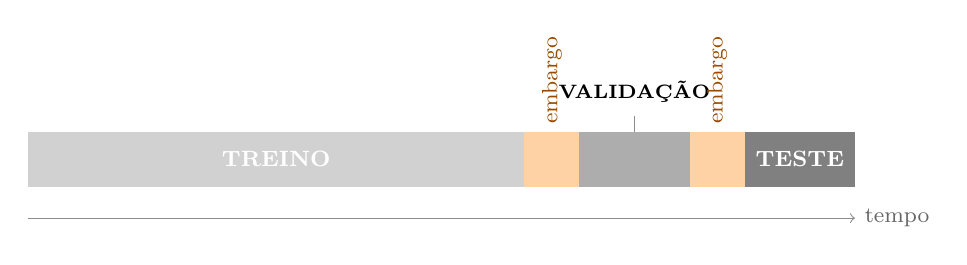
\begin{tikzpicture}[font=\small]
  \fill[black!18] (0,0) rectangle (6.3,0.7);
  \fill[orange!35] (6.3,0) rectangle (7.0,0.7);
  \fill[black!32] (7.0,0) rectangle (8.4,0.7);
  \fill[orange!35] (8.4,0) rectangle (9.1,0.7);
  \fill[black!50] (9.1,0) rectangle (10.5,0.7);
  \node[white, font=\footnotesize\bfseries] at (3.15,0.35) {TREINO};
  % ⚠️ "VALIDAÇÃO" é mais larga do que o seu bloco (1.4 cm) e derramava sobre as duas bandas
  % do embargo, de um lado e do outro. Sai para cima, com um traço a apontar-lhe. Alargar o
  % bloco não servia: as larguras são as proporções reais do eixo do tempo.
  \node[font=\scriptsize\bfseries, anchor=south] (rotval) at (7.7,0.95) {VALIDAÇÃO};
  \draw[black!45] (7.7,0.9) -- (7.7,0.7);
  \node[white, font=\footnotesize\bfseries] at (9.8,0.35) {TESTE};
  \node[orange!60!black, font=\footnotesize, rotate=90] at (6.65,1.35) {embargo};
  \node[orange!60!black, font=\footnotesize, rotate=90] at (8.75,1.35) {embargo};
  \draw[->, black!45] (0,-0.4) -- (10.5,-0.4) node[right, black!60, font=\footnotesize] {tempo};
\end{tikzpicture}
\caption[Divisão temporal com embargo]{A divisão dos dados obedece à \textbf{ordem cronológica} e
não a um sorteio. Entre blocos consecutivos intercala-se um \emph{embargo} de cinco dias, uma vez
que o rótulo de cada notícia depende dos três dias seguintes: sem ele, o final do bloco de treino
seria determinado por dias pertencentes ao bloco seguinte.}
\label{fig:met_divisao}
\end{figure}

O bloco de teste contém mais exemplos do que o de treino. O corte é feito em dias de negociação,
segundo a proporção de setenta, quinze e quinze por cento, e a assimetria resulta da densidade de
notícias, que cresce acentuadamente ao longo do período coberto pelo corpus. A divisão por dias, e
não por número de exemplos, é necessária para que notícias do mesmo dia não sejam repartidas por
blocos distintos.

A pontuação produzida pelo modelo não constitui, por si, uma probabilidade. Uma vez que o valor é
apresentado ao utilizador, é convertido através de calibração \emph{a posteriori}, ajustando uma
sigmoide de dois parâmetros sobre o bloco de validação reservado \autocite{niculescu2005calibration}:

\begin{equation}
p_{\text{calibrada}} = \frac{1}{1 + e^{-(a\,p_{\text{bruta}} + b)}}
\label{eq:platt}
\end{equation}

Os valores aprendidos são $a = 3{,}700$ e $b = -2{,}313$. O sinal negativo de $b$ indica que o
modelo, sem calibração, produz valores sistematicamente superiores à frequência observada. Parte
deste comportamento decorre da reponderação das classes durante o treino, que desloca as pontuações
para cima por construção.

A calibração é ajustada num bloco cuja prevalência de casos positivos difere da do bloco de teste,
consequência da divisão cronológica. O efeito é mensurável e está reportado no
Capítulo~\ref{cap:avaliacao}. A transformação é monótona e preserva a ordenação entre notícias, que
é o que a política de decisão utiliza; o valor absoluto apresentado é o que fica afetado.

\section{Ferramentas e infraestrutura}
\label{sec:met_ferramentas}

O sistema está escrito em Python 3.12. As dependências que produzem os resultados desta dissertação
estão fixadas em versões exatas, e não em intervalos, de modo que o ambiente possa ser recriado
noutra máquina: \texttt{numpy}~2.1.3, \texttt{pandas}~2.2.3, \texttt{scikit-learn}~1.9.0,
\texttt{matplotlib}~3.11.0, \texttt{sentence-transformers}~5.6.0 e \texttt{torch}~2.12.1 na variante
para CPU. Nenhum resultado exige unidade de processamento gráfico, consequência das opções
descritas neste capítulo.

Todas as fontes de dados são gratuitas. Os preços provêm de uma cadeia de fornecedores alternativos
consultados por ordem fixa, uma vez que nenhuma fonte gratuita apresenta fiabilidade suficiente
isoladamente; o sistema regista sempre qual delas respondeu. As notícias provêm de três fornecedores
complementares, cuja comparação é apresentada no Capítulo~\ref{cap:sistema}. A entrega utiliza a
interface de robô do Telegram.

\section{Desafios tecnológicos e sociais}
\label{sec:met_desafios}

Esta secção enuncia os riscos que um sistema com estas características levanta e as decisões de
desenho que respondem a cada um.

\subsection{Privacidade e proteção de dados}
\label{sec:met_privacidade}

Uma carteira de investimentos revela rendimento, aversão ao risco e projetos de vida, informação
que o Regulamento Geral sobre a Proteção de Dados trata como merecedora de proteção reforçada
quando permite traçar o perfil de uma pessoa.

A decisão de desenho que responde a este risco é a minimização: o sistema não conhece as posições
dos utilizadores e não as solicita. Não existe carteira, não existem posições nem montantes, e o
canal público não identifica destinatários. Um alerta sobre uma empresa é idêntico para todos os
leitores. O custo desta opção é a impossibilidade de personalização, uma vez que o sistema alerta
sobre uma lista fixa de empresas e não sobre as posições de quem lê.

Existe uma exceção que importa nomear. Os utilizadores que optem por receber alertas personalizados
através do robô do Telegram ficam associados a dois elementos: o identificador de conversa
atribuído pela plataforma e a lista de empresas selecionadas. Não são armazenados nome, contacto
nem montantes. O tratamento assenta no pedido expresso do próprio utilizador, que o inicia ao
subscrever e o termina através de um comando que elimina o registo.

\subsection{Segurança}
\label{sec:met_seguranca}

Um sistema autónomo que consome serviços externos detém credenciais. As chaves residem em variáveis
de ambiente e no cofre de segredos da plataforma, nunca no repositório, e o texto enviado para os
registos passa por uma função que mascara parâmetros com nome de credencial. Esta segunda
salvaguarda responde ao facto de as mensagens de erro de bibliotecas de comunicação reproduzirem o
endereço do pedido, e de algumas interfaces transportarem a chave nesse endereço.

O codificador de frases é obtido sob pedido e confrontado com uma soma de controlo fixada no
código. Na ausência dessa verificação, um ficheiro corrompido ou substituído modificaria sem aviso
o critério de semelhança utilizado pelo sistema.

\subsection{Questões éticas e sociais}
\label{sec:met_etica}

A restrição fundadora do trabalho é também a sua principal salvaguarda ética. Um sistema que
anunciasse o comportamento futuro do preço emitiria uma previsão não verificável no momento da
leitura; um sistema que indicasse instrumentos a adquirir entraria numa atividade regulada. Esta
fronteira é de desenho, traçada por prudência e não a partir de uma análise do direito aplicável:
não houve parecer jurídico, e a operação do sistema como serviço exigiria obtê-lo previamente.

A garantia aplica-se ao que o sistema escreve e não ao que reproduz. Os títulos de terceiros são
citados na íntegra, uma vez que constituem o facto que desencadeia o alerta e permitem a
verificação na fonte, e alguns são eles próprios especulativos. Daqui decorre uma limitação sem
solução no âmbito assumido: o filtro de relevância determina se um título é sobre a empresa, e não
se é factual. A distinção entre notícia e opinião exigiria um classificador que o sistema não
possui.

A interrupção repetida constitui o segundo risco. O efeito está documentado em sistemas de apoio à
decisão clínica, onde \textcite{ancker2017alertfatigue} medem que a probabilidade de aceitação de um
alerta decresce à medida que o volume de alertas recebidos aumenta, e que o efeito se acentua com a
repetição do mesmo alerta. O domínio é distinto e o que se transfere é o mecanismo: quem é
interrompido com frequência deixa de distinguir as interrupções, momento a partir do qual um aviso
correto e um aviso incorreto passam a ter o mesmo efeito. O sistema responde com um orçamento
diário de alertas, um limiar crescente para alertas repetidos da mesma empresa e supressão de
notícias que reproduzem uma história já comunicada.

O terceiro risco decorre da própria explicação. A confiança em sistemas automáticos falha nos dois
sentidos, com o utilizador a ignorar um aviso correto ou a aceitar um aviso incorreto
\autocite{lee2004trust}, e a presença de uma explicação aumenta a aceitação de respostas erradas
\autocite{bansal2021whole}. O sistema apresenta, por essa razão, os casos passados individualmente,
com data e desfecho, em vez de os resumir a uma média suscetível de ser lida como previsão. Que
esta opção produza confiança apropriada constitui uma hipótese e não um resultado, uma vez que o
estudo com utilizadores necessário para a verificar não foi realizado.
